% ==============================================================================
% PLANTILLA DE INFORME - PFM02 / IIIEPE / MAEM
% ==============================================================================
% Uso:
% 1. Duplica este archivo y renombra la copia por unidad, sesion y actividad.
% 2. Actualiza documenttitle, documentsubtitle, documentsubject, sesionname,
%    activityname, docente y fecha de entrega.
% 3. Lee la consigna del EVA/posgrado y NO pegues las instrucciones completas
%    dentro del producto final. Usa la consigna como lista de cumplimiento.
% 4. Revisa la bibliografia indicada, toma notas, registra citas y redacta con
%    comprension propia.
% 5. Identifica el producto academico o didactico solicitado y construyelo dentro
%    del documento siempre que sea posible.
% 6. Entrega en PDF con la nomenclatura indicada por la unidad de aprendizaje.
%
% Formato institucional recomendado para IIIEPE:
% - Fuente tipo Helvetica, equivalente visual a Arial.
% - Interlineado 1.5.
% - Citas autor-anio con natbib: usar \citep{clave} o \citet{clave}.
% - Referencias en bibliografia BibTeX, formato APA 7 en cuerpo y referencias.
% - Caratula, resumen breve, desarrollo, producto solicitado, conclusion y
%   bibliografia.
% - Redaccion academica clara, coherente, cohesionada, formal y sin faltas.
% - Portada con identidad IIIEPE, programa MAEM, matricula y correo institucional.
% - La portada puede llevar una marca de agua institucional discreta; ajustar
%   las variables coverwatermark... si se requiere apagarla o cambiar intensidad.
%
% Criterios generales de cumplimiento:
% - Responder exactamente a la actividad solicitada en el EVA o por la figura docente.
% - Alinear contenido matematico, PDA, aprendizaje de la secuencia, fases,
%   evaluacion y retroalimentacion.
% - Identificar conceptos, elementos, criterios o categorias de forma precisa.
% - Analizar, interpretar y tomar postura; no solo copiar fuentes.
% - Organizar la informacion por jerarquia, secuencia y criterios claros.
% - Incluir conclusion personal cuando la actividad lo permita o lo solicite.
% - Usar citas y referencias en APA 7.
% - Evitar copiar las indicaciones de la actividad en el cuerpo final.
%
% Regla para productos visuales:
% - Si la actividad pide tabla, cuadro comparativo, esquema, mapa conceptual,
%   mapa mental, linea de tiempo, diagrama, matriz, lista de verificacion, red
%   conceptual, SQA, organizador grafico o producto similar, realizarlo
%   preferentemente con LaTeX/TikZ para mantener nitidez, evidencia editable y
%   diseno controlado.
% - Si la consigna exige Canva, Miro u otra herramienta externa, insertar una
%   captura nitida y conservar la explicacion dentro del documento.
% - Para tablas extensas, usar pagina limpia, sin encabezados ni pies, landscape,
%   letra pequena y restaurar el estilo al terminar.
%
% Criterios de redaccion personal:
% - No escribir para llenar espacio; escribir para sostener una idea.
% - Convertir informacion en criterio: que significa, como funciona, que problema
%   resuelve, que limite presenta y que consecuencia produce.
% - Estructura mental recomendada: problema -> sistema -> consecuencia -> postura.
% - Usar pensamiento de diagnostico: entrada -> proceso -> salida.
% - Cada parrafo debe tener funcion: presentar, explicar, comparar, valorar o
%   concluir.
% - Usar primera persona con moderacion academica: "Considero que",
%   "Desde esta perspectiva", "La posicion que sostengo es". Evitar "yo creo".
%
% Notas de enfoque personal segun enfoque_personal.txt:
% - La voz debe ser academica, tecnica, directa, estrategica y funcional.
% - El texto no debe sonar como estudiante pasivo que recopila: debe sonar como
%   alguien que interpreta, ordena, cruza datos y busca consecuencia practica.
% - Antes de redactar, identificar la funcion de cada seccion: abrir problema,
%   definir criterio, demostrar con evidencia, comparar, valorar o concluir.
% - Evitar frases genericas como "es importante porque si" o "desde siempre".
%   Sustituirlas por relaciones verificables: causa, efecto, limite, costo,
%   funcion, riesgo, implicacion o mejora.
% - Cada concepto debe pasar de definicion a analisis. Formula util:
%   concepto -> funcion -> riesgo si se aplica mal -> consecuencia -> postura.
% - La postura personal no debe ser opinion suelta. Debe tener tres piezas:
%   posicion, razon y efecto. Ejemplo: "Considero que X, porque Y; por ello Z".
% - Integrar experiencia o criterio propio sin perder formalidad: no narrar la
%   vida personal, sino usar mirada practica para explicar por que el tema
%   importa en educacion, derecho, instituciones, comunicacion o profesion.
%
% Estilo observado en actividades ya realizadas:
% - Abrir con una tesis concreta:
%   "La ensenanza de las matematicas no solo transmite procedimientos:
%   organiza formas de razonar, representar y justificar."
% - Formular el problema en negativo y positivo:
%   "El problema no es solo..., sino..."
% - Convertir el producto visual en argumento:
%   "El cuadro no solo recopila datos; reconstruye la funcion, el problema y el
%   punto que requiere correccion."
% - Cerrar con aprendizaje transferible:
%   "No basta con saber que dice la norma; tambien debe analizarse a quien
%   protege, a quien excluye y que razones permiten defenderla publicamente."
%
% Nivel cognitivo esperado:
% - Recordar: usar solo para definir conceptos basicos. No debe ser el nivel
%   dominante en una actividad ponderable.
% - Comprender: explicar con palabras propias y relacionar con el tema.
% - Aplicar: llevar el concepto a un caso, norma, texto, correo, dilema o hecho.
% - Analizar: separar elementos, detectar causas, efectos, tensiones y limites.
% - Evaluar: sostener una postura con criterios, fuentes y consecuencias.
% - Crear: elaborar producto propio: mapa, cuadro, linea de tiempo, ensayo,
%   propuesta, reformulacion, glosario, portafolio o solucion argumentada.
%
% Regla de nivel minimo:
% - Si la actividad vale puntos y pide producto, no quedarse en recordar o
%   comprender. Debe llegar por lo menos a aplicar y analizar; si pide conclusion
%   o postura, debe llegar a evaluar.
%
% Uso de tecnicas didacticas:
% - Esta plantilla conserva el manual "Tecnicas didacticas del aprendizaje" como
%   apoyo para construir productos visuales, analiticos y reflexivos.
% - Cuando la actividad mencione una tecnica didactica, identificar: definicion
%   de la tecnica, producto esperado, pasos de construccion, criterios de revision
%   y cierre reflexivo.
% - La tecnica didactica no debe verse como adorno. Debe mostrar seleccion,
%   jerarquia, relacion entre ideas y lectura propia.
% - Siempre que sea viable, construir la tecnica en LaTeX/TikZ: cuadro
%   comparativo, mapa conceptual, esquema, mapa mental, linea de tiempo, matriz,
%   red conceptual, diagrama de flujo, tabla SQA o lista de verificacion.
%
% Checklist antes de entregar:
% [ ] El titulo, unidad de aprendizaje, sesion, docente y fecha estan actualizados.
% [ ] El objetivo coincide con la consigna del EVA/posgrado.
% [ ] El contenido, PDA y aprendizaje de la secuencia estan alineados.
% [ ] La actividad considera las cinco fases de PFM02 cuando se trate de una secuencia.
% [ ] La practica incluye mecanizacion, variacion y al menos una situacion en contexto.
% [ ] La evaluacion mide el aprendizaje declarado y no solo la repeticion del algoritmo.
% [ ] El producto solicitado aparece visible, rotulado y completo.
% [ ] La introduccion plantea un problema o postura, no solo anuncia el tema.
% [ ] El desarrollo explica, conecta y analiza.
% [ ] Hay citas APA autor-anio dentro del texto.
% [ ] La bibliografia final coincide con las fuentes citadas.
% [ ] La conclusion responde que se comprendio y que postura se sostiene.
% [ ] El nivel cognitivo llega al menos a aplicacion y analisis.
% [ ] Si hay conclusion/postura, incluye posicion, razon y consecuencia.
% [ ] La tecnica didactica solicitada esta construida y explicada.
% [ ] No aparecen instrucciones copiadas de la consigna dentro del producto.
% [ ] Ortografia, acentos, sintaxis y nombres propios revisados.
% [ ] Si se uso IA como apoyo, el texto fue comprendido, revisado y apropiado.
% ==============================================================================

% CREACION DEL DOCUMENTO
\documentclass[
	spanish,
	letterpaper, oneside
]{article}

% ==============================================================================
% INFORMACION DEL DOCUMENTO
% Actualizar en cada actividad.
% Ejemplos:
% \def\documenttitle {Cuadro comparativo de conceptos fundamentales}
% \def\documentsubtitle {Actividad X - Nombre de la asignatura}
% \def\documentsubject {Actividad Semana X}
% ==============================================================================
\def\documenttitle {Titulo de la actividad}
\def\documentsubtitle {PFM02 - Temas selectos de matematicas I}
\def\documentsubject {Informe academico / Secuencia didactica}

\def\documentauthor {Mtro. Martin Jonathan de la Cruz Munoz}
\def\coursename {Temas selectos de matematicas I}
\def\coursecode {PFM02}

\def\universityname {Instituto de Investigacion, Innovacion y Estudios de Posgrado para la Educacion del Estado de Nuevo Leon}
\def\universityfaculty {Maestria en Aprendizaje y Ensenanza de las Matematicas}
\def\universitydepartment {Temas selectos de matematicas I}
\def\universitydepartmentimage {img/iiiepe/marca-iiiepe.png}
\def\universitydepartmentimagecfg {height=1.75cm}
\def\universitylocation {Monterrey, Nuevo Leon}

% DATOS FIJOS DEL POSGRADO
\def\studentfullname {Mtro. Martin Jonathan de la Cruz Munoz}
\def\studentid {00874}
\def\studentemail {martin.delacruz@campus.iiiepe.edu.mx}
\def\institutionurl {https://iiiepe.edu.mx/}
\def\programperiod {1er tetramestre marzo--julio 2026}
\def\programmodality {Modalidad presencial}
\def\programshort {MAEM}
\def\maemsource {https://iiiepe.edu.mx/maestria-en-aprendizaje-y-ensenanza-de-las-matematicas/}
\def\coursegroup {Grupo A}
\def\courseperiod {Marzo--julio 2026}
\def\evaname {EVA posgrado}
\def\activityname {Nombre de la actividad}
\def\sessionname {Sesion por definir}
\def\blockname {Bloque por definir}
\def\methodology {Aprendizaje basado en indagacion}
\def\steamenfoque {STEAM como enfoque}
\def\curriculumsource {Programa Sintetico Fase 6}
\def\formativefield {Saberes y Pensamiento Cientifico}
\def\mainproduct {Informe academico con secuencia didactica matematica}
\def\docentename {Nombre de la figura docente}

% INTEGRANTES, PROFESORES Y FECHAS
\def\authortable {
	\begin{tabular}{ll}
		\textbf{Alumno:}
		& \begin{tabular}[t]{l}
			 \studentfullname \\
		\end{tabular} \\
		Matricula: & \studentid \\
		Correo institucional: & \studentemail \\

		\textit{Figura docente:}
		& \begin{tabular}[t]{l}
			\docentename
		\end{tabular} \\
		Unidad: & \coursename \\
		Clave: & \coursecode \\
		Grupo: & \coursegroup \\
		Sesion/Bloque: & \sessionname\ / \blockname \\
		Actividad: & \activityname \\
		Programa: & \programshort \\
		Periodo: & \courseperiod \\
		& \\
		\multicolumn{2}{l}{Fecha de realizacion: \today} \\
		\multicolumn{2}{l}{\universitylocation}
	\end{tabular}
}

% IMPORTACION DEL TEMPLATE BASE
\input{template}

% FORMATO GENERAL
\usepackage{helvet}
\renewcommand{\familydefault}{\sfdefault}

% IDENTIDAD VISUAL IIIEPE
\definecolor{iiiepeNavy}{HTML}{163B5C}
\definecolor{iiiepeBlue}{HTML}{1F6F9F}
\definecolor{iiiepeAqua}{HTML}{20B7A8}
\definecolor{iiiepeOrange}{HTML}{F28C28}
\definecolor{iiiepePaper}{HTML}{F6F8F7}
\definecolor{iiiepeInk}{HTML}{1E2A32}
\definecolor{iiiepeMuted}{HTML}{667085}
\def\portraittitlecolor {iiiepeNavy}

% TABLAS Y PRODUCTOS VISUALES
\usepackage{array}
\usepackage{longtable}
\usepackage{pdflscape}
\usepackage{tikz}
\usetikzlibrary{
	arrows.meta,
	positioning,
	calc,
	matrix,
	fit,
	shapes.geometric,
	shadows.blur
}

% CITAS EN FORMATO AUTOR-ANIO, COMPATIBLE CON APA 7 EN EL CUERPO DEL TEXTO
% Usar:
% - Cita parentetica: \citep{clave}
% - Cita narrativa: \citet{clave}
% - Varias fuentes: \citep{clave1,clave2}
\setcitestyle{authoryear,open={(},close={)}}

% ==============================================================================
% AYUDAS DE REDACCION
% Quitar o comentar \pendiente cuando el documento final este terminado.
% ==============================================================================
\newcommand{\pendiente}[1]{\textcolor{red}{[PENDIENTE: #1]}}

% ==============================================================================
% MARCA DE AGUA EN PORTADA
% - Se aplica solo a la portada porque usa \AddToShipoutPictureBG*.
% - Para apagarla en alguna actividad: \def\coverwatermarkenabled {false}
% - Usar opacidad baja para que no compita con titulo, datos ni logotipo.
% ==============================================================================
\def\coverwatermarkenabled {true}
\def\coverwatermarkimage {img/iiiepe/logo-puntos.png}
\def\coverwatermarkopacity {0.09}
\def\coverwatermarkwidth {0.58\paperwidth}
\def\coverwatermarkxshift {0cm}
\def\coverwatermarkyshift {-0.15cm}

\newcommand{\insertcoverwatermark}{%
	\ifthenelse{\equal{\coverwatermarkenabled}{true}}{%
		\AddToShipoutPictureBG*{%
			\begin{tikzpicture}[remember picture,overlay]
				\node[
					opacity=\coverwatermarkopacity,
					inner sep=0pt,
					xshift=\coverwatermarkxshift,
					yshift=\coverwatermarkyshift
				] at (current page.center) {%
					\includegraphics[width=\coverwatermarkwidth]{\coverwatermarkimage}%
				};
			\end{tikzpicture}%
		}%
	}{}%
}

\begin{document}

% PORTADA
\insertcoverwatermark
\templatePortrait

% CONFIGURACION DE PAGINA Y ENCABEZADOS
\templatePagecfg
\onehalfspacing

% ==============================================================================
% RESUMEN / ABSTRACT
% Debe ser breve. Formula recomendada:
% Tema + objetivo + tecnica/producto + enfoque personal.
% ==============================================================================
\begin{abstractd}
	\textbf{Objetivo:} \pendiente{Redactar el objetivo con verbo academico: analizar, disenar, aplicar, evaluar, argumentar o proponer. En PFM02 debe vincularse con un contenido matematico, un PDA y una evidencia de aprendizaje.}

	\textbf{Producto elaborado:} \pendiente{Indicar si el producto es informe, secuencia didactica, tabla, banco de ejercicios, analisis de sesion, recurso matematico, evaluacion, rubrica o reflexion docente.}

	\textbf{Enfoque de analisis:} \pendiente{Enunciar el criterio de lectura: contenido matematico + representacion + procedimiento + contexto + evaluacion. Debe mostrar como la actividad favorece comprension y no solo mecanizacion.}

	\textbf{Nivel cognitivo:} \pendiente{Indicar el nivel dominante: aplicar, analizar, evaluar o crear. Para secuencias didacticas, el nivel esperado suele llegar a crear porque se disena una propuesta propia con intencion pedagogica.}
\end{abstractd}

% TABLA DE CONTENIDOS - INDICE
\templateIndex

% CONFIGURACIONES FINALES
\templateFinalcfg

% ======================= INICIO DEL DOCUMENTO =======================

% ==============================================================================
% SECCION 1: INTRODUCCION
% Apertura recomendada:
% - Iniciar con una afirmacion clara, no con una frase generica.
% - Traducir la consigna a un problema academico, didactico, matematico,
%   pedagogico o profesional, segun la unidad de aprendizaje.
% - Explicar por que importa.
% - Cerrar anticipando el enfoque personal.
% ==============================================================================
\section{Introduccion}

\pendiente{Abrir con una afirmacion propia sobre el contenido matematico de la actividad. Ejemplo: "La ensenanza de los numeros con signo no puede reducirse a memorizar reglas; requiere construir referencias, relaciones de orden y sentido en situaciones reales".}

\pendiente{Explicar el problema didactico que atiende la actividad: conversion entre representaciones, comprension de operaciones, uso de signos, interpretacion de unidades, volumen, dificultad de lenguaje matematico, evaluacion o transferencia a contexto.}

\pendiente{Cerrar con la postura inicial: que criterio guiara el informe y que evidencia permitira sostener que hubo aprendizaje matematico.}

% ==============================================================================
% SECCION OPCIONAL: IDENTIDAD DEL PROGRAMA
% Conservar cuando el informe requiera contextualizar la actividad en la MAEM.
% Puede comentarse en entregas breves.
% ==============================================================================
\section{Contexto institucional y formativo}

\subsection{Datos del programa}

La actividad se desarrolla en el marco de la \universityfaculty, adscrita al
\universityname. El programa corresponde a una formacion de posgrado orientada a
fortalecer la reflexion, el diseno, la implementacion y la evaluacion de
propuestas didacticas para la ensenanza y el aprendizaje de las matematicas.

\subsection{Sentido formativo de la MAEM}

La \programshort\ coloca la practica docente como objeto de analisis profesional:
no basta con resolver una consigna, sino que es necesario reconocer que problema
educativo se atiende, que criterio teorico o didactico se usa, que evidencia se
produce y que mejora puede derivarse para el aula.

\subsection{Base academica del curso PFM02}

La unidad de aprendizaje \coursecode\ --\coursename-- se orienta al analisis y
diseno de actividades para contenidos matematicos escolares. Su eje de trabajo
consiste en articular el contenido, el proceso de desarrollo de aprendizaje, la
explicacion didactica, la practica, la evaluacion y la retroalimentacion.

De acuerdo con el enfoque observado en los materiales de la unidad, la
secuencia didactica se organiza en cinco momentos: conocimientos previos,
explicacion o exploracion del contenido, practica con mecanizaciones y
situaciones en contexto, evaluacion y retroalimentacion. Esta estructura permite
que el informe no se limite a presentar ejercicios, sino que explique la
intencion matematica y pedagogica de cada decision.

\subsection{Referencia curricular}

Cuando la actividad se relacione con secundaria, se recomienda revisar el
\curriculumsource, especialmente el campo \formativefield. Este documento
funciona como punto de partida curricular: define contenidos y procesos de
desarrollo de aprendizaje, pero exige contextualizacion docente para convertirlos
en actividades pertinentes para un grupo real \citep{sepFase6}.

% Para insertar la malla curricular oficial en una actividad que lo requiera:
% \begin{figure}[H]
% 	\centering
% 	
\includegraphics[width=0.85\linewidth]{img/iiiepe/maem-plan-estudios.png}
% 	\caption{Plan de estudios de la Maestria en Aprendizaje y Ensenanza de las Matematicas.}
% \end{figure}

\subsection{Datos del estudiante}

\begin{itemize}
	\item Alumno: \studentfullname.
	\item Matricula: \studentid.
	\item Correo institucional: \studentemail.
	\item Modalidad: \programmodality.
	\item Unidad de aprendizaje: \coursecode\ -- \coursename.
	\item Grupo y periodo: \coursegroup, \courseperiod.
\end{itemize}

% ==============================================================================
% SECCION 2: DESARROLLO / ANALISIS
% Adaptar los subtitulos segun la unidad de aprendizaje y la consigna.
%
% Productos posibles:
% - Cuadro comparativo: criterios, evidencia, diferencia, valoracion.
% - Mapa conceptual: concepto central, conceptos secundarios, conectores claros.
% - Linea de tiempo: fecha/etapa, hecho, aporte, consecuencia.
% - Secuencia didactica: contenido, PDA, fase, actividad, evidencia y evaluacion.
% - Estudio de caso: situacion, elementos, problema, interpretacion, solucion.
% - Lista de verificacion: criterio observable, indicador, cumplimiento, mejora.
% - Glosario: concepto, definicion, funcion, ejemplo, fuente.
% - Reporte o ensayo: tesis, argumentos, evidencia, postura y cierre.
%
% Regla de parrafo:
% Entrada: concepto o problema.
% Proceso: explicacion, fuente y relacion.
% Salida: consecuencia, criterio o postura.
% ==============================================================================
\section{Desarrollo}

\subsection{Contexto y problema didactico}

\pendiente{Presentar la actividad, sesion o contenido matematico. Convertir la consigna en problema didactico: que dificultad suele presentar el aprendizaje, que representacion se necesita, que error frecuente debe anticiparse y que evidencia demostrara comprension.}

\subsection{Contenido, PDA y aprendizaje de la secuencia}

\begin{longtable}{@{}p{0.25\linewidth}p{0.68\linewidth}@{}}
	\caption{Ficha base para actividades de PFM02}\label{tab:ficha-pfm02}\\
	\toprule
	\textbf{Elemento} & \textbf{Descripcion para completar} \\
	\midrule
	\endfirsthead
	\toprule
	\textbf{Elemento} & \textbf{Descripcion para completar} \\
	\midrule
	\endhead
	Tema de la sesion & \pendiente{Ejemplo: conversion de fracciones a decimales, suma y resta de fracciones, operaciones con enteros, volumen de prismas y piramides.} \\
	Contenido matematico & \pendiente{Escribir el contenido curricular o matematico que se abordara. Debe ser preciso y no demasiado amplio.} \\
	PDA & \pendiente{Registrar el proceso de desarrollo de aprendizaje correspondiente. Si se usa Fase 6, citar el documento curricular.} \\
	Aprendizaje de la secuencia & \pendiente{Redactar con verbo observable: resolver, convertir, justificar, comparar, calcular, modelar, argumentar o interpretar.} \\
	Evidencia esperada & \pendiente{Indicar que producto mostrara el aprendizaje: procedimiento, tabla, problema resuelto, explicacion, recurso, evaluacion, rubrica o reflexion.} \\
	Criterio de evaluacion & \pendiente{Senalar como se distinguira una respuesta correcta de una comprension suficiente: procedimiento, argumento, unidades, signo, representacion y sentido del resultado.} \\
	\bottomrule
\end{longtable}

\subsection{Mapa de contenidos base}

Los materiales revisados para PFM02 muestran una progresion centrada en
contenidos fundamentales de secundaria: representacion de numeros racionales,
operaciones con fracciones, numeros con signo y medicion geometrica. La tabla
siguiente sirve como guia para contextualizar futuras actividades.

\begin{longtable}{@{}p{0.16\linewidth}p{0.26\linewidth}p{0.30\linewidth}p{0.20\linewidth}@{}}
	\caption{Referentes de contenido para PFM02}\label{tab:contenidos-pfm02}\\
	\toprule
	\textbf{Sesion} & \textbf{Tema} & \textbf{Contenido/PDA de referencia} & \textbf{Evidencia sugerida} \\
	\midrule
	\endfirsthead
	\toprule
	\textbf{Sesion} & \textbf{Tema} & \textbf{Contenido/PDA de referencia} & \textbf{Evidencia sugerida} \\
	\midrule
	\endhead
	01 & Conversion fraccion--decimal & Expresion de fracciones como decimales y de decimales como fracciones; uso de diversas estrategias de conversion. & Conversiones justificadas y comparacion de estrategias. \\
	02 & Suma y resta con fracciones & Extension del significado de las operaciones y sus relaciones inversas al resolver problemas. & Problemas con procedimiento, equivalencias y explicacion. \\
	03A & Multiplicacion y division con fracciones & Uso de operaciones con fracciones en situaciones problematicas; cuidado con reglas sin significado. & Ejercicios graduados y situacion contextualizada. \\
	03B & Operaciones con enteros & Extension a numeros positivos y negativos; uso del cero como referencia. & Recta numerica, balance, temperatura o profundidad. \\
	11A & Volumen de prismas y piramides & Medicion y calculo en diferentes contextos; uso de estrategias para calcular volumen. & Problemas con formulas, unidades e interpretacion. \\
	\bottomrule
\end{longtable}

\subsection{Marco conceptual}

\pendiente{Explicar los conceptos centrales con fuentes. No acumular definiciones: cada concepto debe mostrar funcion, limite, ejemplo de aula o consecuencia para el aprendizaje. En PFM02 conviene distinguir concepto, procedimiento, representacion y uso contextual.}

\subsection{Nivel cognitivo aplicado}

\pendiente{Explicar brevemente que operacion cognitiva exige la actividad. En una secuencia PFM02 no basta con recordar formulas: se espera aplicar procedimientos, analizar errores, evaluar estrategias y crear una organizacion didactica propia.}

\subsection{Producto solicitado}

\pendiente{Insertar aqui el producto solicitado por la actividad: informe, secuencia didactica, matriz, banco de ejercicios, recurso matematico, analisis de sesion, evaluacion, rubrica, tabla o reflexion. Si es visual, realizarlo en LaTeX/TikZ siempre que sea posible.}

\subsection{Modelo de secuencia didactica}

\begin{longtable}{@{}p{0.17\linewidth}p{0.25\linewidth}p{0.25\linewidth}p{0.20\linewidth}@{}}
	\caption{Matriz editable de secuencia didactica PFM02}\label{tab:secuencia-pfm02}\\
	\toprule
	\textbf{Fase} & \textbf{Actividad docente} & \textbf{Actividad del estudiante} & \textbf{Evidencia} \\
	\midrule
	\endfirsthead
	\toprule
	\textbf{Fase} & \textbf{Actividad docente} & \textbf{Actividad del estudiante} & \textbf{Evidencia} \\
	\midrule
	\endhead
	1. Conocimientos previos & \pendiente{Plantear pregunta detonadora, diagnostico breve o problema inicial.} & \pendiente{Explicar estrategias conocidas, anticipar resultados o resolver un caso simple.} & \pendiente{Registro de saberes previos, respuestas o errores iniciales.} \\
	2. Explicacion/exploracion & \pendiente{Modelar el contenido con representaciones, ejemplos y contraejemplos.} & \pendiente{Registrar pasos, justificar decisiones y formular dudas.} & \pendiente{Apuntes, ejemplo guiado, tabla o representacion.} \\
	3. Practica & \pendiente{Proponer mecanizaciones, variaciones y situaciones en contexto.} & \pendiente{Resolver, comparar estrategias y explicar procedimientos.} & \pendiente{Ejercicios resueltos, problemas contextualizados y justificacion.} \\
	4. Evaluacion & \pendiente{Aplicar instrumento: examen breve, rubrica, laboratorio, exposicion, autoevaluacion o coevaluacion.} & \pendiente{Demostrar desempeno mediante procedimiento correcto y explicacion.} & \pendiente{Producto evaluable con criterios claros.} \\
	5. Retroalimentacion & \pendiente{Devolver criterios, corregir errores frecuentes y orientar mejora.} & \pendiente{Reconocer logro, dificultad, estrategia util y siguiente paso.} & \pendiente{Reflexion metacognitiva o plan de mejora.} \\
	\bottomrule
\end{longtable}

\subsection{Tecnica o estrategia didactica aplicada}

\pendiente{Cuando la actividad indique una tecnica didactica, explicar aqui como se uso. En PFM02 puede justificarse la estrategia desde la indagacion: antecedente, pregunta, exploracion, formalizacion, practica, evaluacion y metacognicion.}

% ==============================================================================
% BLOQUE OPCIONAL: TABLA O CUADRO COMPARATIVO AMPLIO
% Usar cuando el producto necesite mucho ancho:
% - \clearpage para iniciar en pagina limpia.
% - \pagestyle{empty} para quitar encabezado y pie en el producto amplio.
% - landscape para aprovechar el ancho horizontal.
% - scriptsize, tabcolsep y arraystretch para controlar legibilidad.
% - Restaurar \pagestyle{fancy} al terminar.
%
% Si la tabla es corta, puede omitirse landscape y usarse longtable normal.
% ==============================================================================
% \clearpage
% \pagestyle{empty}
% \begin{landscape}
% \begingroup
% \scriptsize
% \setlength{\tabcolsep}{4pt}
% \renewcommand{\arraystretch}{1.35}
% \begin{longtable}{@{}p{0.18\linewidth}p{0.39\linewidth}p{0.39\linewidth}@{}}
% \caption{Titulo del cuadro comparativo}\label{tab:cuadro-comparativo}\\
% \toprule
% \textbf{Criterio} & \textbf{Elemento 1} & \textbf{Elemento 2} \\
% \midrule
% \endfirsthead
% \toprule
% \textbf{Criterio} & \textbf{Elemento 1} & \textbf{Elemento 2} \\
% \midrule
% \endhead
% Concepto & \pendiente{Contenido sintetico con cita si aplica.} & \pendiente{Contenido sintetico con cita si aplica.} \\
% Caracteristicas & \pendiente{Contenido.} & \pendiente{Contenido.} \\
% Funcion & \pendiente{Contenido.} & \pendiente{Contenido.} \\
% Valoracion critica & \pendiente{Contenido.} & \pendiente{Contenido.} \\
% \bottomrule
% \end{longtable}
% \endgroup
% \end{landscape}
% \pagestyle{fancy}

% ==============================================================================
% BLOQUE OPCIONAL: PRODUCTO VISUAL EN TIKZ
% Usar para mapa conceptual, mapa mental, esquema, flujo, proceso o diagrama.
% Cada flecha debe expresar relacion; no usar nodos sueltos sin conectores.
% ==============================================================================
% \begin{figure}[H]
% 	\centering
% 	\begin{tikzpicture}[
% 		node distance=1.3cm,
% 		box/.style={rectangle, rounded corners=2pt, draw=black!65, fill=black!4, align=center, minimum width=3.2cm, minimum height=0.9cm},
% 		arrow/.style={-{Latex[length=2.5mm]}, thick, draw=black!65}
% 	]
% 		\node[box] (centro) {Concepto central};
% 		\node[box, right=of centro] (relacion) {Concepto relacionado};
% 		\node[box, below=of relacion] (efecto) {Consecuencia};
%
% 		\draw[arrow] (centro) -- node[above]{implica} (relacion);
% 		\draw[arrow] (relacion) -- node[right]{produce} (efecto);
% 	\end{tikzpicture}
% 	\caption{Titulo del producto visual.}
% \end{figure}

\subsection{Analisis propio}

\pendiente{Explicar que muestra el producto, que criterio se sostiene y que aprendizaje se obtiene. En PFM02 conviene usar la secuencia: dificultad matematica -> decision didactica -> evidencia de aprendizaje -> mejora posible.}

\subsection{Aplicacion a la practica docente}

\pendiente{Explicar como el analisis o producto puede transferirse a la ensenanza de las matematicas: grupo, contenido, dificultad, representacion, estrategia, evidencia de aprendizaje y mejora esperada.}

\subsection{Lista de verificacion PFM02}

Antes de entregar, revisar que la actividad cumpla los siguientes criterios:

\begin{itemize}
	\item El tema, contenido, PDA y aprendizaje de la secuencia estan alineados.
	\item La introduccion plantea un problema didactico, no solo anuncia el tema.
	\item La explicacion matematica distingue concepto, procedimiento y representacion.
	\item La practica incluye ejercicios directos y al menos una situacion en contexto.
	\item La dificultad progresa de lo guiado a lo autonomo.
	\item La evaluacion mide el aprendizaje declarado y permite revisar errores.
	\item La retroalimentacion incluye una pregunta metacognitiva o plan de mejora.
	\item Las operaciones, signos, unidades, formulas y resultados fueron verificados.
	\item Las fuentes consultadas aparecen citadas en el texto y en bibliografia.
\end{itemize}

% ==============================================================================
% SECCION 3: POSTURA PERSONAL
% Debe mostrar comprension real. No repetir fuentes; interpretar.
% ==============================================================================
\section{Postura personal}

\pendiente{Redactar una postura academica y moderada. Relacionar el tema con PFM02, la formacion docente y la ensenanza de las matematicas. Formula recomendada: "Considero que una secuencia de matematicas es pertinente cuando...", "La razon es...", "La consecuencia didactica de esto es...".}

% ==============================================================================
% SECCION 4: CONCLUSION
% Cierre recomendado:
% - Responder directamente a la actividad.
% - Indicar que se comprendio, no solo que se elaboro.
% - Mencionar criterio personal final.
% - No introducir informacion nueva.
% ==============================================================================
\section{Conclusion}

\pendiente{Cerrar con sintesis, aprendizaje y postura final. Debe responder que se aprendio sobre el contenido matematico y que criterio docente se fortalece para disenar nuevas actividades.}

% ==============================================================================
% MANUAL DE TECNICAS DIDACTICAS
% Dejar incluido en la plantilla maestra. En una entrega final, puede comentarse
% esta linea si la docente solo solicita el producto de la semana.
% ==============================================================================
% ==============================================================================
% MANUAL OPERATIVO: TECNICAS DIDACTICAS DEL APRENDIZAJE
% Fuente de referencia: Coleccion "100 Tecnicas Didacticas de Ensenanza y
% Aprendizaje", Fasciculos 1 a 5, UnADM, 2023.
%
% Proposito del archivo:
% - Servir como guia para elegir, construir y revisar productos didacticos.
% - Traducir la tecnica solicitada en un producto LaTeX/TikZ verificable.
% - Evitar entregas genericas: todo producto debe tener estructura, criterio,
%   analisis y postura cuando la actividad lo permita.
%
% Regla general para nuevas actividades:
% Si la planeacion pide tabla, cuadro comparativo, mapa conceptual, mapa mental,
% linea de tiempo, diagrama, esquema, matriz, cronologia, red conceptual,
% histograma, flujo o proceso, construirlo preferentemente con TikZ/LaTeX.
% Usar captura externa solo si la consigna exige una herramienta especifica o si
% el producto requiere una plataforma interactiva.
% ==============================================================================

\clearpage
\section{Manual operativo de técnicas didácticas}

\subsection{Regla base para productos visuales}

Cuando la actividad solicite un producto visual, el producto debe construirse como parte del documento y no como un elemento improvisado. La regla de trabajo es: si el producto puede representarse con nodos, flechas, tablas, matrices, líneas, ciclos, mapas o relaciones, debe elaborarse en TikZ o con entornos LaTeX como \texttt{tabular}, \texttt{longtable} o \texttt{figure}. Esto permite controlar formato, legibilidad, jerarquía, citas, continuidad visual y coherencia con el documento.

El producto no debe funcionar como adorno. Debe demostrar comprensión: seleccionar información, jerarquizarla, relacionarla y cerrar con una lectura propia. En términos prácticos, cada producto debe contestar cuatro preguntas: qué organiza, con qué criterios lo organiza, qué relación muestra y qué conclusión permite sostener.

\subsection{Estructura común de las técnicas UnADM}

Los fascículos de \textit{100 Técnicas Didácticas de Enseñanza y Aprendizaje} trabajan cada técnica con una lógica estable: definición, estructura, utilidad, proceso de construcción, consideraciones y referencias. Para convertir esa lógica en una actividad universitaria, se recomienda usar esta secuencia:

\begin{enumerate}
	\item \textbf{Identificar el producto solicitado.} No es lo mismo comparar, explicar, analizar, sintetizar o construir. El verbo de la consigna define el nivel de profundidad.
	\item \textbf{Determinar los elementos obligatorios.} Toda técnica tiene piezas mínimas: categorías, conceptos, fuentes, etapas, actores, criterios, datos, ejemplos o conclusiones.
	\item \textbf{Elegir el formato TikZ/LaTeX.} Tabla para comparar, nodos para mapas, flechas para procesos, línea horizontal para cronologías, matriz para decisiones.
	\item \textbf{Redactar antes de diseñar.} El diseño no corrige una idea débil. Primero se definen conceptos y relaciones; después se dibuja.
	\item \textbf{Agregar lectura crítica.} El producto debe mostrar qué significa la información, por qué importa y cómo se aplica.
	\item \textbf{Cerrar con postura.} Si la actividad pide conclusión, debe responder de forma directa la pregunta final y justificarla.
\end{enumerate}

\subsection{Taxonomía de ejecución}

La colección clasifica las técnicas por nivel de ejecución. Esta lectura ayuda a decidir qué profundidad debe tener la entrega:

\begin{longtable}{@{}p{0.14\linewidth}p{0.2\linewidth}p{0.56\linewidth}@{}}
\toprule
\textbf{Nivel} & \textbf{Acción} & \textbf{Criterio para la actividad} \\
\midrule
\endhead
1 & Recordar & Recuperar datos, conceptos, nombres o hechos. Requiere precisión, pero no basta para una actividad universitaria completa. \\
2 & Explicar & Aclarar el significado de un concepto y su función. Debe incluir ejemplos o aplicación. \\
3 & Aplicar & Usar el conocimiento en una situación, caso, norma o problema. Debe mostrar procedimiento. \\
4 & Analizar & Separar elementos, identificar causas, efectos, relaciones y límites. Exige postura crítica. \\
5 & Sintetizar & Integrar información dispersa en un producto ordenado. Debe mostrar jerarquía y selección. \\
6 & Construir & Crear un producto, propuesta, estrategia, guion, ensayo, proyecto o solución. Exige diseño completo y justificación. \\
\bottomrule
\end{longtable}

\subsection{Manual por producto frecuente}

\subsubsection*{Cuadro comparativo}

Usar cuando la consigna pida comparar corrientes, autores, normas, escuelas, conceptos, textos, versiones o modelos. Debe contener una tabla con conceptos en columnas y categorías en filas. Las categorías no deben ser genéricas: deben permitir contraste real. Para asignaturas de Derecho se recomiendan categorías como concepto, fundamento, autores, principios, función, aplicación, límites y valoración crítica; para Redacción en contextos virtuales conviene usar claridad, coherencia, cohesión, formalidad, objetividad, adecuación al receptor y efecto comunicativo.

\textbf{Construcción:} investigar, seleccionar información relevante, definir categorías, ordenar por jerarquía, redactar celdas breves pero sustanciales, citar fuentes y cerrar con conclusión personal. En TikZ/LaTeX puede hacerse con \texttt{longtable}; si se requiere diseño más visual, usar nodos en matriz.

\textbf{Revisión:} cada fila debe permitir una comparación inmediata; si una categoría no cambia la comprensión, se elimina o se reemplaza.

\subsubsection*{Cuadro sinóptico}

Sirve para organizar un tema de lo general a lo particular. Debe mostrar niveles: tema central, categorías principales, subcategorías y detalles. Es útil para corrientes filosóficas, clasificación de derechos, teorías de justicia o tipos de normas.

\textbf{Construcción:} definir tema central, extraer categorías, ordenar por dependencia lógica y usar llaves, ramas o cajas. En TikZ se recomienda una estructura de árbol con nodos alineados.

\subsubsection*{Mapa conceptual}

Debe mostrar conceptos y relaciones mediante palabras de enlace. No basta con poner cajas conectadas; cada flecha debe decir qué relación existe: causa, implica, deriva, limita, permite, exige, se opone a, fundamenta.

\textbf{Construcción:} seleccionar concepto central, jerarquizar conceptos principales y secundarios, escribir conectores precisos, evitar saturación visual y cerrar con explicación breve del mapa. En TikZ usar nodos jerárquicos con flechas etiquetadas.

\subsubsection*{Mapa mental}

Funciona para explorar asociaciones desde una idea central. A diferencia del mapa conceptual, admite ramas más libres, colores, imágenes o palabras clave. Es útil para lluvia de ideas, conceptos iniciales o planeación de investigación.

\textbf{Construcción:} ubicar idea central, crear ramas principales, agregar subramas, usar palabras breves y cerrar con una interpretación. En TikZ usar nodos radiales o coordenadas polares.

\subsubsection*{Línea de tiempo y cronología ilustrada}

La línea de tiempo organiza eventos por secuencia temporal; la cronología ilustrada agrega apoyo visual o iconográfico. Sirve para evolución del pensamiento jurídico, historia de derechos, reformas constitucionales o desarrollo de una corriente.

\textbf{Construcción:} seleccionar fechas relevantes, ordenar cronológicamente, resumir cada evento, señalar causa o consecuencia y cerrar con lectura histórica. En TikZ usar una línea horizontal con hitos alternados arriba/abajo.

\subsubsection*{Esquema}

El esquema resume una estructura lógica. Puede ser jerárquico, secuencial, causal o temático. Sirve cuando la actividad pide explicar un tema sin llegar a mapa conceptual.

\textbf{Construcción:} identificar tema, dividirlo en partes, ordenar relaciones y redactar con frases breves. En TikZ usar cajas alineadas o árbol simple.

\subsubsection*{Diagrama de flujo}

Representa pasos, decisiones y resultados. Es útil para procedimientos jurídicos, interpretación normativa, juicio de amparo, análisis de caso o toma de decisiones.

\textbf{Construcción:} definir inicio, pasos, decisiones, salidas y cierre. Usar rombos para decisiones, rectángulos para acciones y flechas para secuencia. En TikZ usar \texttt{shapes.geometric} y flechas \texttt{Stealth}.

\subsubsection*{Diagrama de Venn}

Muestra coincidencias y diferencias entre conjuntos. Funciona para comparar derecho/moral, legalidad/justicia, reglas/principios o corrientes filosóficas.

\textbf{Construcción:} definir conjuntos, colocar rasgos exclusivos y zona de intersección. En TikZ usar círculos semitransparentes.

\subsubsection*{Diagrama de Gowin}

Relaciona pregunta central, conceptos, principios, registros, transformaciones y conclusiones. Es útil para analizar un problema de investigación o una norma desde teoría y evidencia.

\textbf{Construcción:} formular pregunta, colocar teoría de un lado y evidencia del otro, derivar conclusión. En TikZ se puede construir con una V central y bloques laterales.

\subsubsection*{Mapa de cajas, mapa semántico y redes conceptuales}

Estos productos organizan conceptos por agrupaciones, campos de significado o conexiones. Son útiles para conceptos jurídicos fundamentales o familias de teorías.

\textbf{Construcción:} agrupar por criterio, no por ocurrencia. Cada caja o nodo debe tener función. En TikZ usar cajas por bloque, colores moderados y flechas solo cuando exista relación real.

\subsubsection*{Mapeo de procesos}

Sirve para describir un sistema operativo: entradas, actividades, responsables, controles y salidas. En Derecho puede aplicarse a etapas de interpretación, aplicación normativa o solución de controversias.

\textbf{Construcción:} definir entrada, proceso, control, salida y retroalimentación. En TikZ usar flujo horizontal o carriles.

\subsubsection*{Gráfico estadístico e histograma}

Usar cuando existan datos cuantitativos. No inventar cifras. Si no hay datos confiables, no usar gráfico estadístico como decoración.

\textbf{Construcción:} definir variable, fuente, escala, unidades y lectura del dato. En LaTeX puede usarse \texttt{tikzpicture} o \texttt{pgfplots} si se habilita el paquete.

\subsubsection*{SQA}

SQA organiza tres momentos: qué sé, qué quiero saber y qué aprendí. Es útil para iniciar y cerrar una investigación.

\textbf{Construcción:} usar tabla de tres columnas. La última columna debe mostrar aprendizaje nuevo, no repetir la primera.

\subsubsection*{Valoración de decisiones}

Permite comparar alternativas con criterios cualitativos o cuantitativos. Es útil para justificar una postura entre corrientes, métodos interpretativos o soluciones de caso.

\textbf{Construcción:} definir alternativas, establecer criterios, asignar pesos, valorar y justificar la decisión. En LaTeX usar tabla o matriz ponderada.

\subsubsection*{Ensayo, informe, artículo, monografía y reporte de investigación}

Son productos escritos. No requieren TikZ salvo que incorporen figuras. Deben tener estructura: introducción con problema, desarrollo con fuentes y análisis, conclusión con postura, y referencias.

\textbf{Construcción:} planteamiento, marco conceptual, análisis, aplicación, postura y cierre. Evitar texto enciclopédico. La voz debe convertir información en criterio.

\subsubsection*{Reseña, resumen, reporte de lectura, sumillado y exegética}

Son productos de lectura y síntesis. Deben demostrar comprensión del texto fuente, no sustituirlo por paráfrasis superficial.

\textbf{Construcción:} identificar tesis, argumentos, conceptos clave, límite del texto y lectura personal. Citar correctamente.

\subsubsection*{Debate, foro, panel, mesa redonda, controversia y suasoria}

Son productos argumentativos. Requieren postura, contraargumentos y cierre. En Derecho son útiles para defender interpretaciones o criterios.

\textbf{Construcción:} tesis, argumentos, evidencia, objeción, respuesta y conclusión. Si se presenta por escrito, usar subtítulos claros.

\subsubsection*{Estudio de caso, análisis de hechos y noticia falsa}

Estos productos trabajan con hechos. Deben distinguir hecho, interpretación, norma/principio, problema y solución.

\textbf{Construcción:} hechos relevantes, problema central, criterios de análisis, aplicación, postura y consecuencia.

\subsubsection*{Cartel, afiche, anuncio, fotomontaje y videocápsula}

Son productos comunicativos y visuales. Si la entrega es PDF, el cartel o afiche puede construirse con TikZ. Si se requiere video, el documento debe incluir guion, enlace, captura y justificación.

\textbf{Construcción:} objetivo, público, mensaje central, jerarquía visual, fuentes y cierre. No saturar texto.

\subsubsection*{Glosario colaborativo}

Debe incluir término, definición propia, fuente, ejemplo y comentario. No basta copiar definiciones.

\textbf{Construcción:} ordenar alfabéticamente o por familias conceptuales; citar fuentes; agregar aplicación jurídica.

\subsubsection*{Portafolio de evidencias digital}

Integra productos y reflexión sobre el proceso. Debe mostrar trayectoria, no solo acumulación.

\textbf{Construcción:} índice, evidencias, explicación de cada evidencia, aprendizaje, correcciones y conclusión.

\subsubsection*{Simulación, sociodrama, juego de roles, juego de negocios y taller}

Son técnicas de actuación o aplicación. Si se entregan por escrito, deben incluir guion, roles, contexto, desarrollo, resultados y reflexión.

\textbf{Construcción:} problema, roles, reglas, escena o dinámica, decisiones, cierre y aprendizaje.

\subsubsection*{Consulta pública, encuesta, grupos focales y entrevista}

Son técnicas de recolección de información. Requieren objetivo, participantes, instrumento, resultados y análisis.

\textbf{Construcción:} delimitar problema, formular preguntas claras, aplicar, organizar resultados, interpretar y cerrar con hallazgos.

\subsection{Catálogo de las 100 técnicas}

\begin{longtable}{@{}p{0.08\linewidth}p{0.35\linewidth}p{0.16\linewidth}p{0.31\linewidth}@{}}
\toprule
\textbf{No.} & \textbf{Técnica} & \textbf{Nivel} & \textbf{Producto sugerido en LaTeX/TikZ} \\
\midrule
\endhead
1 & Cuadro comparativo & Sintetizar & Longtable o matriz TikZ. \\
2 & Cuadro sinóptico & Sintetizar & Árbol jerárquico TikZ. \\
3 & Cuestionario & Explicar & Tabla de preguntas/respuestas. \\
4 & Debate & Aplicar & Guion argumentativo. \\
5 & Diagrama de Gowin & Aplicar & Diagrama V en TikZ. \\
6 & Ejemplificación & Explicar & Tabla concepto-ejemplo-aplicación. \\
7 & Entrevista & Aplicar & Guion y matriz de hallazgos. \\
8 & Esquema & Sintetizar & Cajas jerárquicas TikZ. \\
9 & Glosario colaborativo & Explicar & Tabla término-definición-fuente. \\
10 & Historieta & Recordar & Viñetas TikZ o guion. \\
11 & Informe & Sintetizar & Documento con secciones. \\
12 & Línea de tiempo & Sintetizar & Timeline TikZ. \\
13 & Mapa conceptual & Sintetizar & Nodos y conectores TikZ. \\
14 & Panel de discusión & Aplicar & Tabla de posturas. \\
15 & Pensamiento de diseño & Recordar & Fases empatizar-definir-idear-prototipar-evaluar. \\
16 & Phillips 66 & Aplicar & Matriz grupo-idea-síntesis. \\
17 & Resumen & Recordar & Texto breve estructurado. \\
18 & Simulación & Construir & Escenario, variables y resultados. \\
19 & Sociodrama & Aplicar & Guion de escenas. \\
20 & Trabajo cooperativo & Aplicar & Plan de roles y evidencias. \\
21 & Análisis de contenido & Analizar & Matriz texto-idea-función-crítica. \\
22 & Análisis de tergiversación textual & Analizar & Tabla afirmación/evidencia/corrección. \\
23 & Análisis y consensos & Analizar & Matriz de acuerdos y disensos. \\
24 & Autoexplicación & Explicar & Secuencia pregunta-respuesta-criterio. \\
25 & Cronología ilustrada & Construir & Línea de tiempo con iconos. \\
26 & Estructuras textuales & Analizar & Mapa de estructura argumentativa. \\
27 & Estudio de casos & Explicar & Hechos-problema-norma-solución. \\
28 & Exposición oral & Aplicar & Guion o diapositivas. \\
29 & Foro & Aplicar & Entrada, réplica y cierre. \\
30 & Grupos de discusión & Aplicar & Matriz de aportaciones. \\
31 & Grupos focales & Explicar & Guion y síntesis de hallazgos. \\
32 & Mapa de cajas & Sintetizar & Cajas agrupadas TikZ. \\
33 & Mapa mental & Explicar & Nodos radiales TikZ. \\
34 & Monografía & Explicar & Documento de investigación. \\
35 & Preguntas y premios & Recordar & Banco de reactivos. \\
36 & Reporte de lectura general & Explicar & Ficha de lectura ampliada. \\
37 & Reseña & Sintetizar & Valoración crítica breve. \\
38 & Rompecabezas & Construir & Integración por piezas. \\
39 & Sumillado & Sintetizar & Texto con notas marginales. \\
40 & Testimonio & Recordar & Entrevista y relato analizado. \\
41 & Consulta pública & Aplicar & Instrumento y matriz de resultados. \\
42 & Controversia estructurada & Analizar & Tesis, antítesis y síntesis. \\
43 & Debate público & Aplicar & Guion de argumentación. \\
44 & Diagrama de Venn & Analizar & Círculos TikZ. \\
45 & Diario de aprendizaje & Recordar & Bitácora reflexiva. \\
46 & Discusión de gabinete & Analizar & Tabla de roles y decisiones. \\
47 & Documentales & Explicar & Guion audiovisual. \\
48 & Encuesta interactiva & Aplicar & Instrumento y gráfica. \\
49 & Ensayo & Construir & Texto argumentativo. \\
50 & Estudio de noticia falsa & Analizar & Verificación y contraste de fuentes. \\
51 & Exegética & Recordar & Interpretación textual guiada. \\
52 & Fábula & Recordar & Narración con moraleja. \\
53 & Heurística de Bruner & Analizar & Ruta descubrimiento-concepto. \\
54 & Histograma & Analizar & Gráfico de frecuencias. \\
55 & Pensamiento analógico & Aplicar & Analogía y transferencia. \\
56 & Poesía lírica & Construir & Producto creativo con reflexión. \\
57 & Sesión bibliográfica & Analizar & Fichas por fuente. \\
58 & SQA & Recordar & Tabla sé-quiero-aprendí. \\
59 & Suasoria & Aplicar & Discurso persuasivo. \\
60 & Tablón de anuncios & Sintetizar & Muro informativo o tablero. \\
61 & Afiche & Explicar & Cartel breve en TikZ. \\
62 & Análisis de hechos & Analizar & Hechos-causas-consecuencias. \\
63 & Anuncio publicitario & Explicar & Pieza persuasiva. \\
64 & Atributos & Explicar & Tabla de cualidades. \\
65 & Diagrama de flujo & Sintetizar & Flujo TikZ. \\
66 & Diálogos simultáneos & Aplicar & Guion de interacción. \\
67 & Feynman & Explicar & Explicación simple y prueba. \\
68 & Gráfico estadístico & Analizar & Gráfico con fuente. \\
69 & Lluvia de ideas dirigida & Explicar & Mapa radial o lista clasificada. \\
70 & Mapa semántico & Sintetizar & Red de significados TikZ. \\
71 & Mapeo de procesos & Analizar & Proceso entrada-salida. \\
72 & Mesa redonda con interrogador & Aplicar & Matriz de preguntas/posturas. \\
73 & Mnemotecnia & Recordar & Reglas de memoria. \\
74 & Portafolio de evidencias digital & Construir & Índice de evidencias. \\
75 & Redes conceptuales & Sintetizar & Grafo TikZ. \\
76 & Reporte de investigación & Explicar & Documento con método. \\
77 & Simposio & Aplicar & Programa y síntesis. \\
78 & Socioaprendizaje & Aplicar & Comunidad y evidencias. \\
79 & Tuits & Sintetizar & Microargumentos. \\
80 & Valoración de decisiones & Analizar & Matriz ponderada. \\
81 & Artículo & Analizar & Texto con tesis y fuentes. \\
82 & Cartel & Explicar & Cartel TikZ. \\
83 & Demostración silenciosa & Aplicar & Secuencia visual. \\
84 & Descripción de un personaje & Aplicar & Perfil estructurado. \\
85 & Estudio intercalado & Aplicar & Plan de estudio espaciado. \\
86 & Examen práctico & Aplicar & Evidencia de ejecución. \\
87 & Fotomontaje digital & Construir & Composición visual justificada. \\
88 & Instrucción personalizada & Analizar & Ruta de aprendizaje individual. \\
89 & Journal digital & Construir & Bitácora digital. \\
90 & Juego de negocios & Analizar & Simulación estratégica. \\
91 & Juego de roles & Aplicar & Guion de roles. \\
92 & Práctica distribuida & Aplicar & Calendario de práctica. \\
93 & Preguntas dirigidas & Construir & Banco de preguntas guía. \\
94 & Proyectos colaborativos & Construir & Plan de proyecto. \\
95 & Reportaje & Construir & Investigación narrativa. \\
96 & Scamper & Recordar & Matriz sustituir-combinar-adaptar. \\
97 & Social media & Aplicar & Estrategia de publicación. \\
98 & Taller & Aplicar & Secuencia de actividades. \\
99 & Videocápsula & Sintetizar & Guion y storyboard. \\
100 & Visitas guiadas virtuales 360 & Construir & Guion, secuencia y recorrido. \\
\bottomrule
\end{longtable}

\subsection{Plantillas TikZ mínimas}

Estas plantillas se pueden copiar a la actividad concreta y ajustar.

\subsubsection*{Mapa conceptual}

\begin{verbatim}
\begin{figure}[H]
\centering
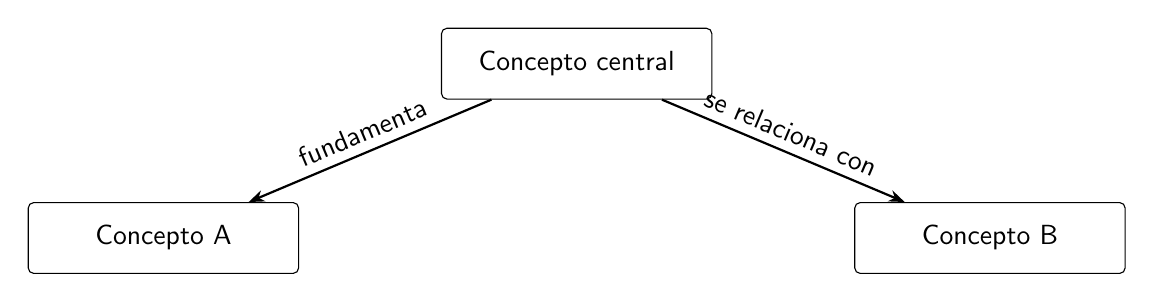
\begin{tikzpicture}[
  concepto/.style={rectangle, draw, rounded corners=2pt,
    align=center, text width=3.2cm, minimum height=0.9cm},
  flecha/.style={-{Stealth[length=2mm]}, thick}
]
\node[concepto] (a) {Concepto central};
\node[concepto, below left=1.3cm and 1.8cm of a] (b) {Concepto A};
\node[concepto, below right=1.3cm and 1.8cm of a] (c) {Concepto B};
\draw[flecha] (a) -- node[above, sloped]{fundamenta} (b);
\draw[flecha] (a) -- node[above, sloped]{se relaciona con} (c);
\end{tikzpicture}
\caption{Mapa conceptual de [tema]}
\end{figure}
\end{verbatim}

\subsubsection*{Línea de tiempo}

\begin{verbatim}
\begin{figure}[H]
\centering
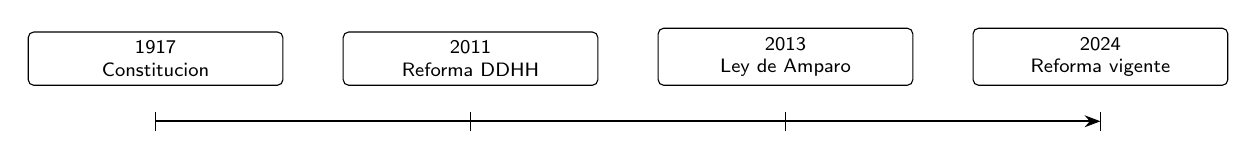
\begin{tikzpicture}[
  evento/.style={rectangle, draw, rounded corners=2pt,
    align=center, text width=3cm, font=\scriptsize},
  eje/.style={-{Stealth[length=2mm]}, thick}
]
\draw[eje] (0,0) -- (12,0);
\foreach \x/\anio/\texto in {
  0/1917/Constitucion,
  4/2011/Reforma DDHH,
  8/2013/Ley de Amparo,
  12/2024/Reforma vigente}
{
  \draw (\x,0.12) -- (\x,-0.12);
  \node[evento, above=0.45cm] at (\x,0) {\anio\\\texto};
}
\end{tikzpicture}
\caption{Linea de tiempo de [tema]}
\end{figure}
\end{verbatim}

\subsubsection*{Diagrama de flujo}

\begin{verbatim}
\begin{figure}[H]
\centering
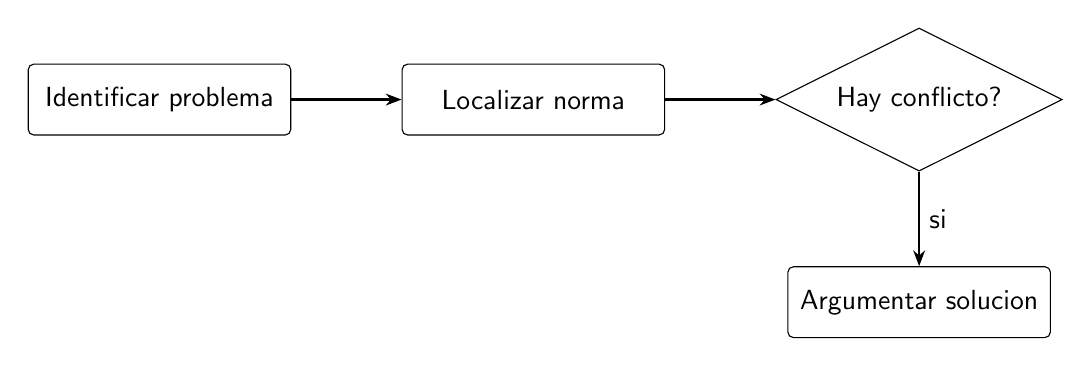
\begin{tikzpicture}[
  paso/.style={rectangle, draw, rounded corners=2pt,
    align=center, text width=3.1cm, minimum height=0.9cm},
  decision/.style={diamond, draw, aspect=2, align=center,
    text width=2.8cm, inner sep=1pt},
  flecha/.style={-{Stealth[length=2mm]}, thick}
]
\node[paso] (inicio) {Identificar problema};
\node[paso, right=1.4cm of inicio] (norma) {Localizar norma};
\node[decision, right=1.4cm of norma] (decision) {Hay conflicto?};
\node[paso, below=1.2cm of decision] (analisis) {Argumentar solucion};
\draw[flecha] (inicio) -- (norma);
\draw[flecha] (norma) -- (decision);
\draw[flecha] (decision) -- node[right]{si} (analisis);
\end{tikzpicture}
\caption{Diagrama de flujo de [proceso]}
\end{figure}
\end{verbatim}

\subsection{Cierre operativo}

La elección de una técnica no debe ser decorativa. Si la actividad pide un producto, la técnica funciona como una herramienta de análisis. El criterio de calidad es que el producto permita ver una decisión intelectual: qué se seleccionó, cómo se organizó, qué relación se construyó y qué postura se puede defender a partir de esa organización.


% BIBLIOGRAFIA
% Cambiar o agregar archivos .bib segun la unidad/actividad.
% Ejemplo: \bibliography{IIIEPE,PFM02}
\nocite{iiiepeMAEM,iiiepeSitio,sepFase6,nctmPrinciplesActions}
\bibliography{IIIEPE,PFM02,UnADM}

% FIN DEL DOCUMENTO
\end{document}
